\documentclass[11pt,a4paper]{article}
\usepackage[margin=25mm]{geometry}
\usepackage{amsmath,amssymb,pdfpages,hyperref}
\pdfinclusioncopyfonts=1
\begin{document}
\thispagestyle{empty}
\begin{center}
{\LARGE Suzuki matrices and a chiral polytope}\par\vspace{10pt}
{\large Complete treatment of the fixed F003 source}\par\vspace{12pt}
Human Compression project
\end{center}
\bigskip
This volume treats the four-page preprint
\emph{On the rank of Suzuki polytopes: an answer to Hubard and
Leemans}, arXiv:2010.04080v1, 8 October 2020.

The first manuscript identifies the error in its matrix classification,
proves the corrected matrix criterion, and retains its six algebraic
cases and final generation argument with their exact hypotheses.

The second manuscript is the unchanged accepted construction of a
chiral rank-four polytope of type $\{31,31,25\}$ with automorphism
group $\operatorname{Sz}(32768)$. It refutes the source's principal
theorem. Its exact finite-field certificate and prior mathematical
reviews are retained by reference; the acquisition is not repeated.

The source conclusions are distinguished from explicitly attributed
structural and reconstruction premises. This volume does not assign
a compression factor, add a second refutation, or claim Lean
verification. Completion concerns the specified source edition and
does not assert a classification of all Suzuki chiral polytopes.

\vfill
The machine-readable claim ledger and exact dependency list accompany
the TeX sources. General proofs remain subject to distinct mathematical
review until the review record is sealed.
\clearpage
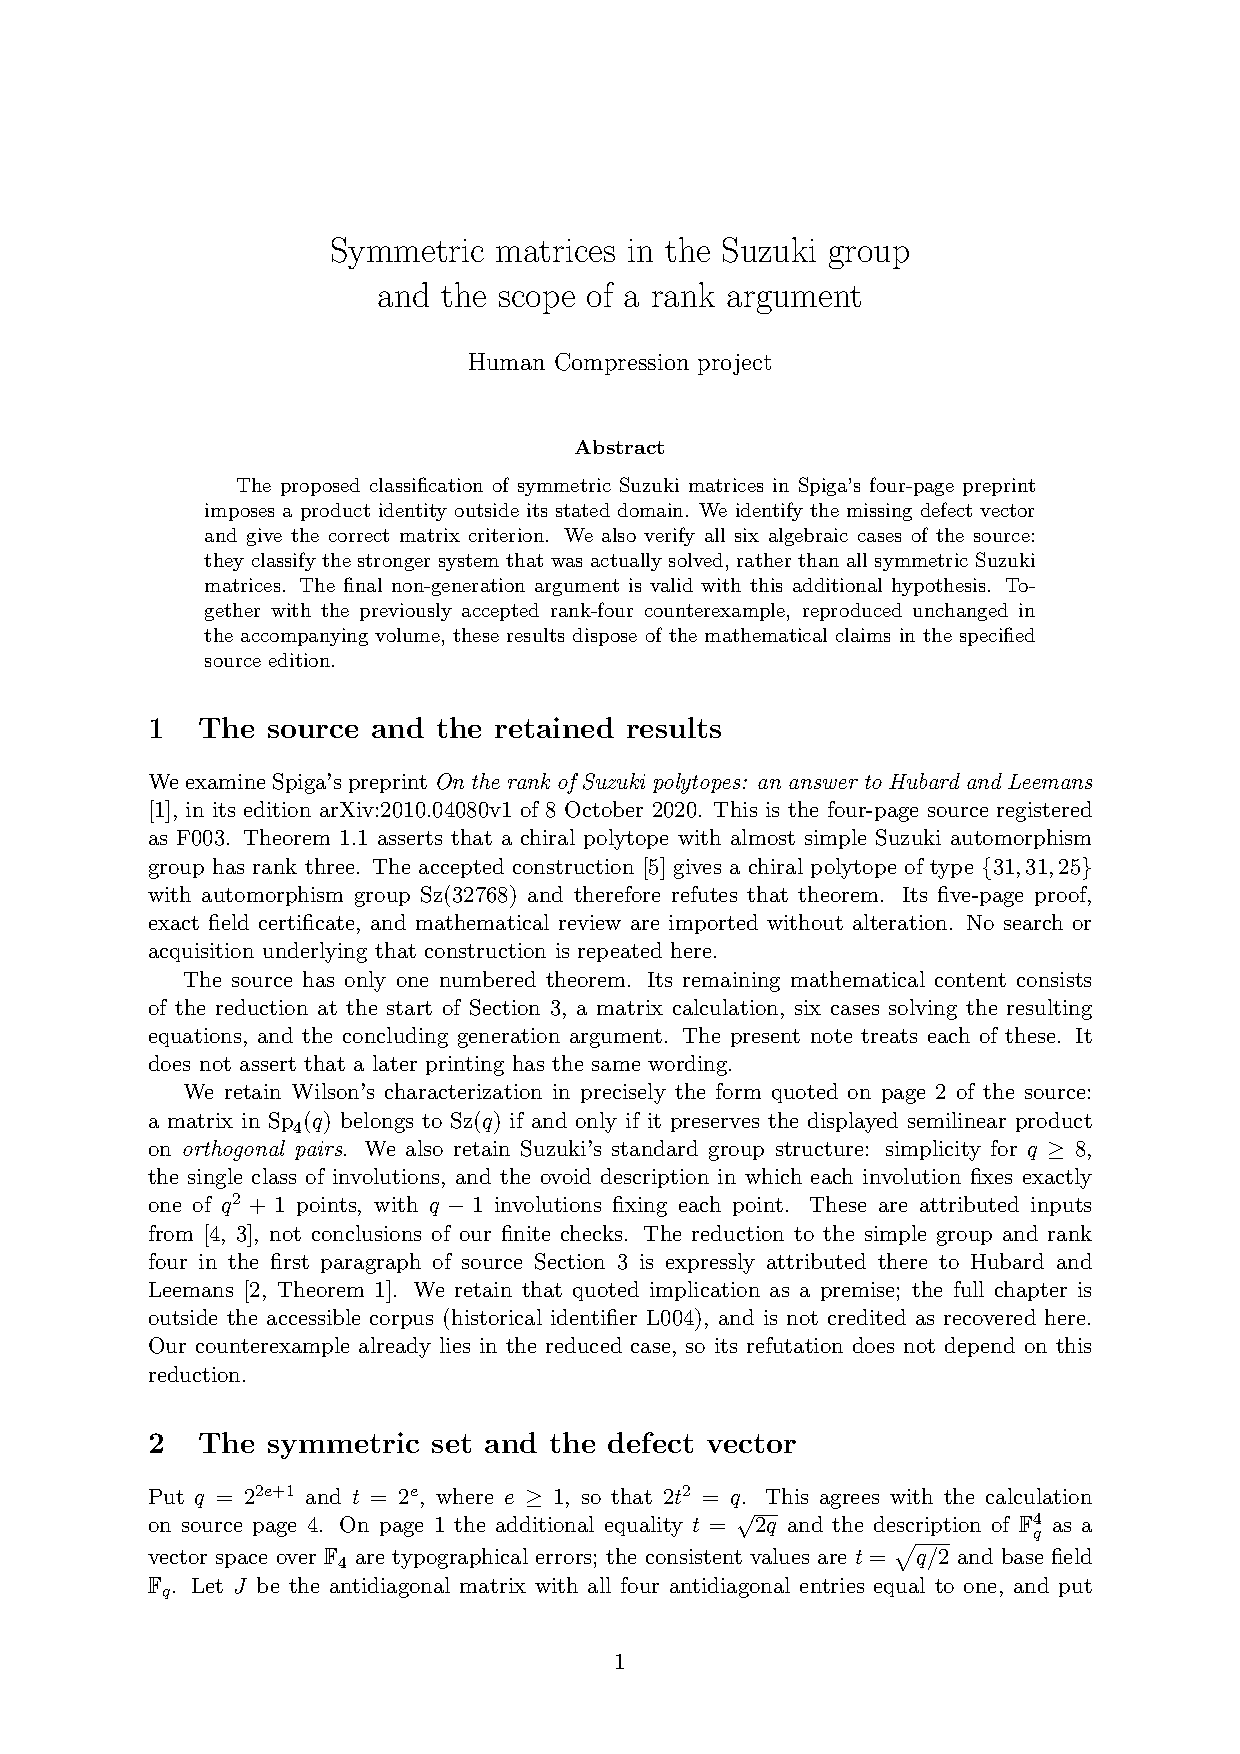
\includepdf[pages=-]{symmetric.pdf}
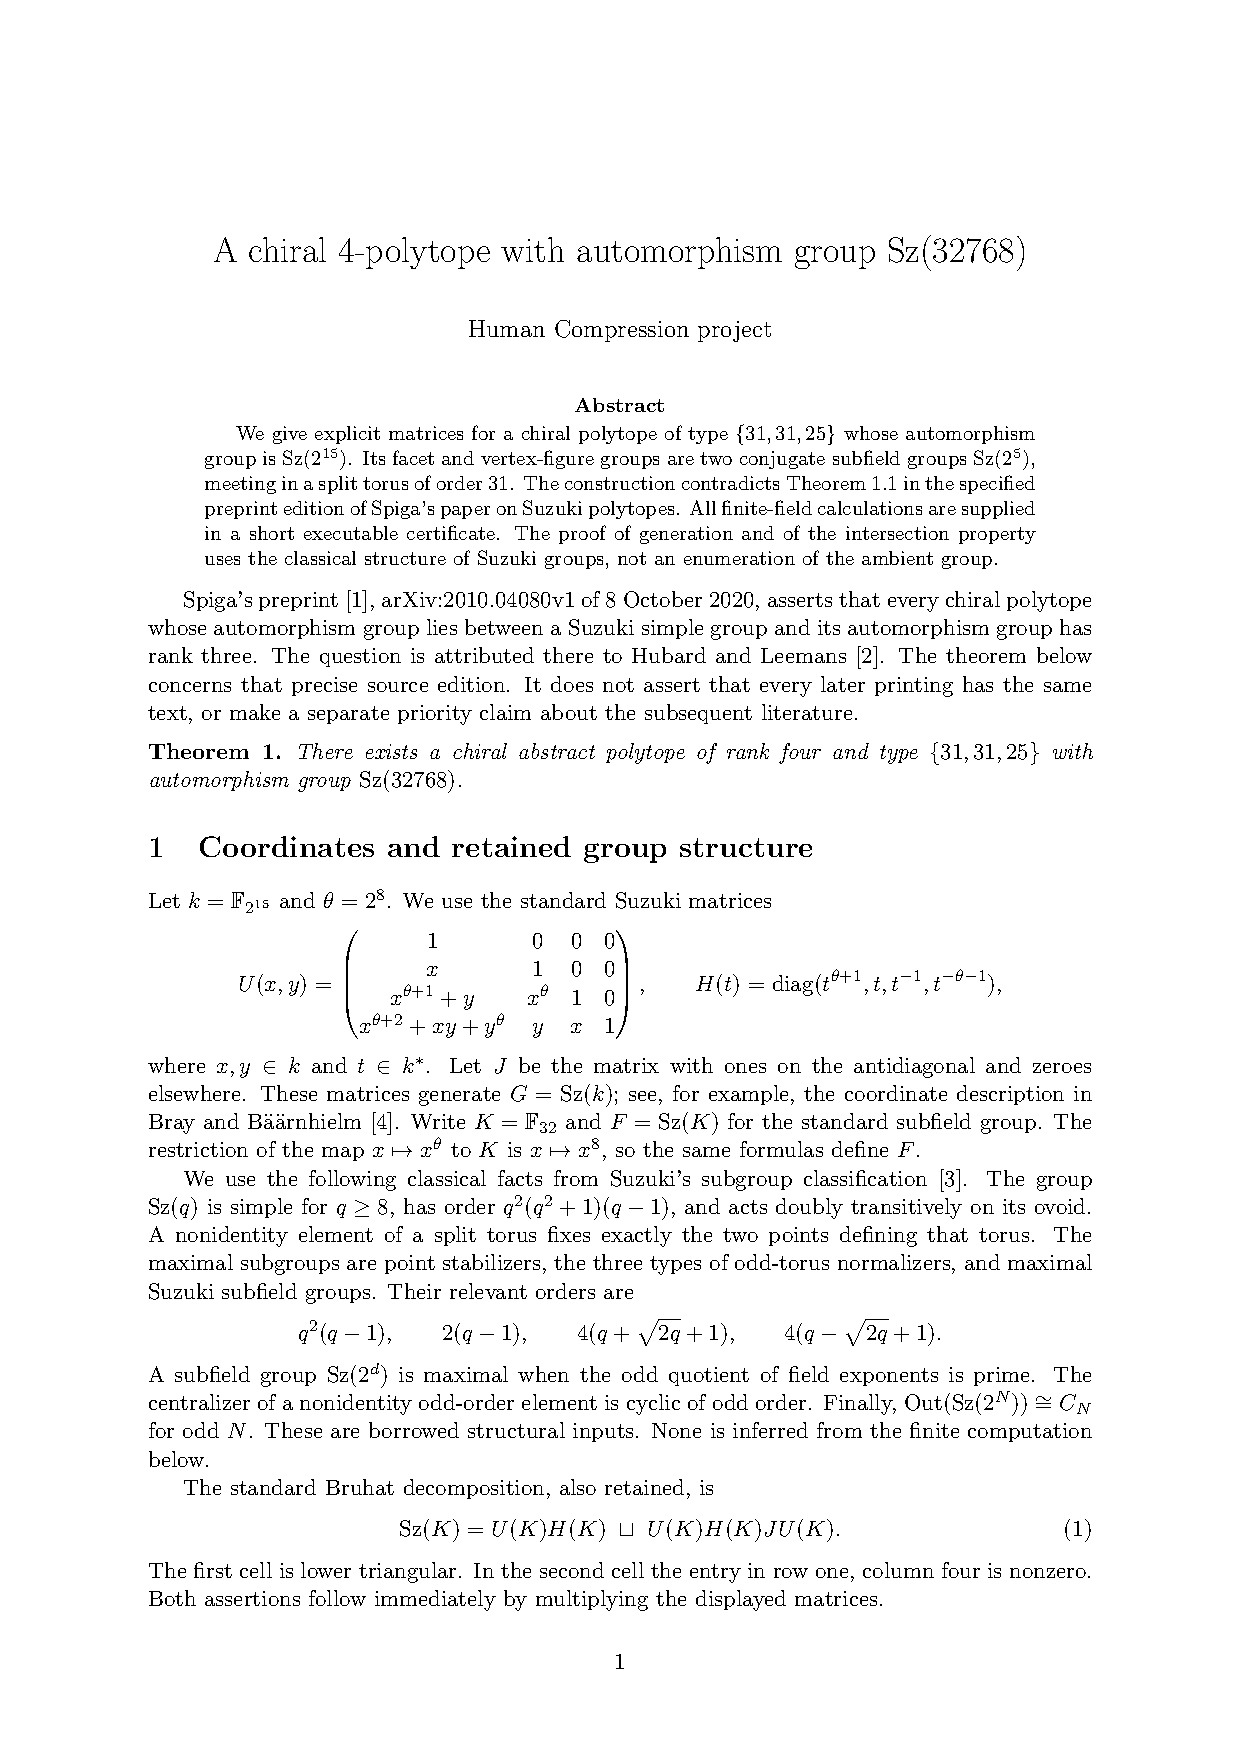
\includepdf[pages=-]{proofs/principal.pdf}
\end{document}
